\documentclass[16pt]{beamer}


\usepackage[frenchb]{babel}
\usepackage[T1]{fontenc}
\usepackage[latin1]{inputenc}
\usepackage{ulem}
\usepackage{graphicx}
%\usetheme{theme/beamerthememetropolis}
\usepackage{theme/beamerthememetropolis}

\usepackage{wrapfig}

\title[Code Talkers]{Navajo Code Talkers}
\date{\today}
\author{Am�lie Risi \& Eric Sageloli}

\begin{document}


\begin{frame}
	\maketitle
\end{frame}
% ------------------------------------------------------------------------------------------------

\section{Introduction}
\begin{frame}
    \frametitle{How to secretly send a message?}

    \begin{itemize}
	\item<1-> steganography %�, hiding the message 
	\item<2-> cryptography %, transforming the message into an apparent nonsense with the possibility to recover the message for selected persons 
    \end{itemize}

    \pause
    \pause
      But also..

    \begin{itemize}
	\item translation of the message into an obscure language
    \end{itemize}
	\begin{figure}
	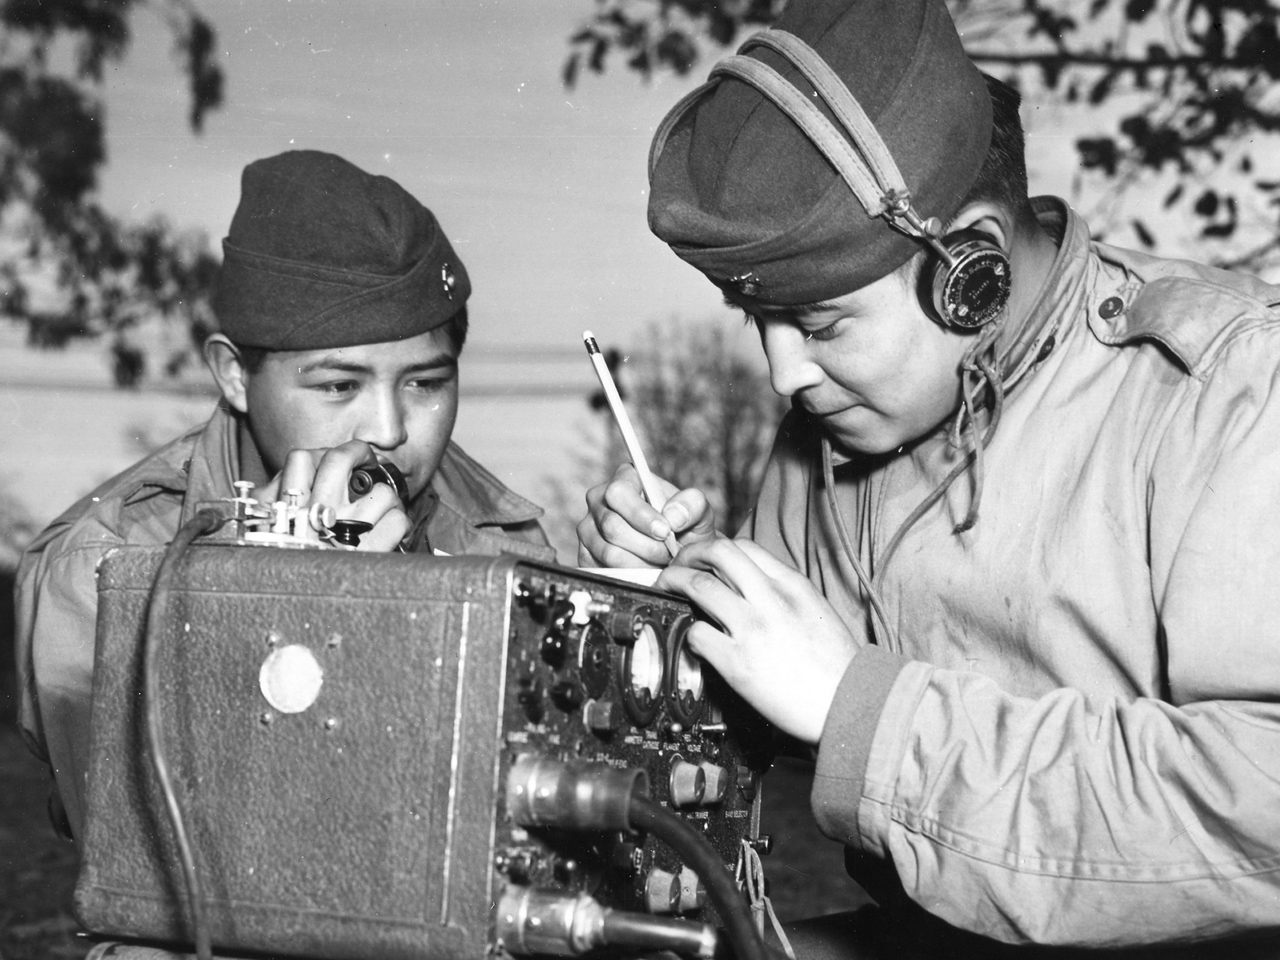
\includegraphics[width=0.5\textwidth]{pictures/title.jpg} 
	\end{figure}
\end{frame}
% ------------------------------------------------------------------------------------------------

\begin{frame}
    \frametitle{Code talkers appeared in the first half of 20th century}
    %This method have been used during the first halt of the 20th century by people, called code talkers, who transmit by radio secret messages during wartime. 
    %This method was particularly used by America which recruit native
    %American who used their native language. 

    Meeting of two conditions:\par
    \begin{itemize}
	\item The existence of the radio and the phone 
	\item By that time, most of the cipher machines were too slow and fragile  
	to be used for tactical field communications 
    \end{itemize}

	\begin{figure}
	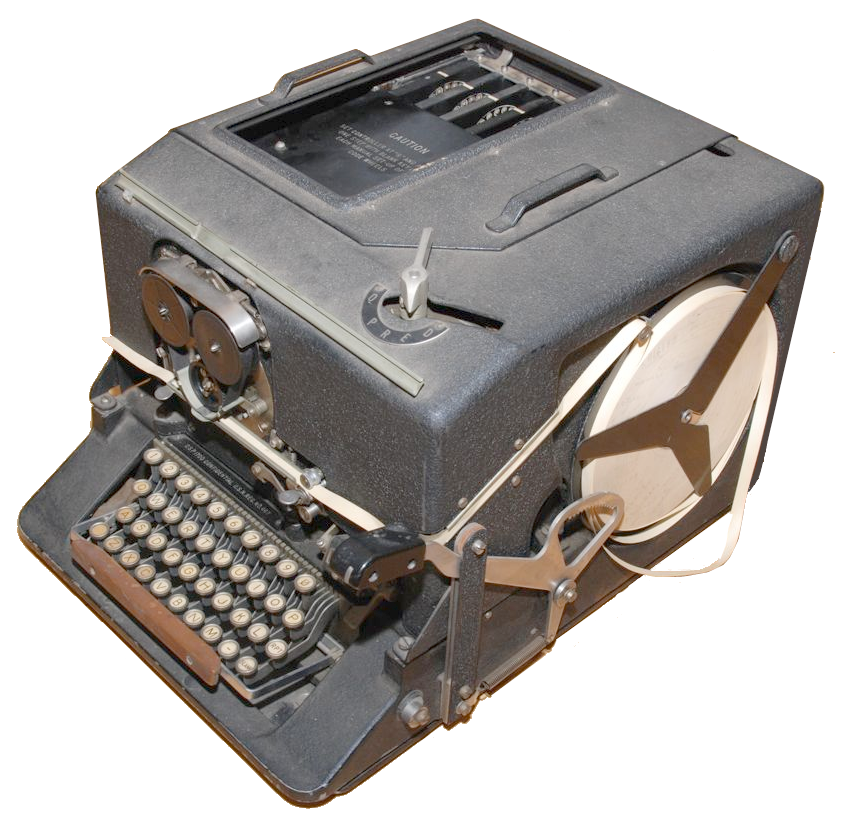
\includegraphics[width=0.3\textwidth]{pictures/SIGABA.png} 
	\caption{The SIGABA}
	\end{figure}

\end{frame}
% ------------------------------------------------------------------------------------------------

\begin{frame}
      \frametitle{Plan}

    Plan:
    \begin{itemize}
	\item relation between the Navajos and the US in the late  of the 19th century
	\item how Navajo code talkers have been recruited
	\item study of the Navajo code. 
    \end{itemize}
\end{frame}
% ------------------------------------------------------------------------------------------------

\begin{frame}
\section{Navajos and US in the late of the 19th century}
    \begin{itemize}
    \item The long walk
    \item Boarding schools 
    \end{itemize}
\end{frame}

\subsection{The Long Walk (1984)}
\begin{frame}
    \frametitle{The long walk}
    In 1864:
    \begin{itemize}
        \item  deportation of approximately 8000 Navajo people by the
	       government of the United States of America
	\item forced trek over 480km into the Bosque Redondo camp.
    \end{itemize}
     
    \pause
    They were not informed of: 
    \begin{itemize} 
	\item where they were going 
	\item why they were being relocated 
	\item how long it would take to get there. 
    \end{itemize}

    \pause
	\vspace{0.4cm}
    \begin{itemize} 
	\item The journey lasted 18 days
	\item Nearly 2000 Navajos died %of exposure to elements and starvations 
    \end{itemize}

\end{frame}
% ------------------------------------------------------------------------------------------------

\subsection{Boarding schools }
\begin{frame}
    \frametitle{Boarding schools}

	around 1900:  many American Indian children were in 
     church-operated boarding schools.


	\begin{figure}
	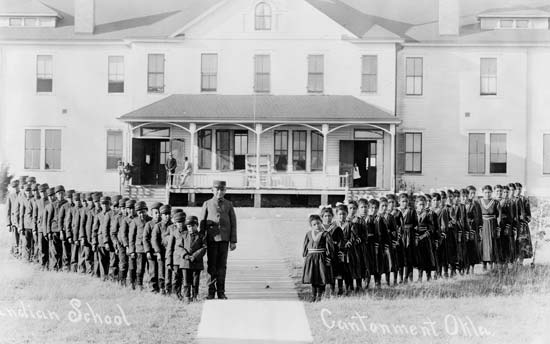
\includegraphics[width=0.5\textwidth]{pictures/boarding_schools.jpg} 
	\end{figure}
\end{frame}
% ------------------------------------------------------------------------------------------------

\begin{frame}
    They were forced to
    \begin{itemize}
	\item speak in English %instead of their native language
	\item give up their traditional clothing
	\item drop their traditional native names 
	\item become Christian
    \end{itemize}
	\vspace{1cm}
\end{frame}
% ------------------------------------------------------------------------------------------------


\begin{frame}
\section{Navajos as code talkers: how they have been recruited}
    \begin{itemize}
	\item Preliminary: the code talkers during the WWI
	\item Pacific war and the idea of Philip Johnston
	\item The demonstration
	\item Efficiency of the Navajos code talkers
    \end{itemize}
\end{frame}
% ------------------------------------------------------------------------------------------------

\begin{frame}
    \frametitle{Preliminary: the code talkers during the WWI}
    \begin{itemize}
    \item First use of native American code talkers : Cherokee. 
    \end{itemize}
	    
    September 1918: During the Second Battle of the Somme, They helped 
 	to win the battle.
\pause
	\begin{itemize}
		\item After WWI,  Germany sent students and
    anthropologists in America in order to study the various tribal dialects of
    American Indians.
	\end{itemize}


\end{frame}  
% ------------------------------------------------------------------------------------------------


\begin{frame}
    \frametitle{Pacific war and the idea of Philip Johnston}

   % \begin{itemize} 
%	\item December 7 1941: Attack on Pearl Harbor
%	\item Pacific war: 7 December 1941 - 2 September 1945		
%    \end{itemize}

    % ![Philip Johnston](pictures/Jonhston.jpg)
     

    Philip Jonhston
	\begin{figure}
	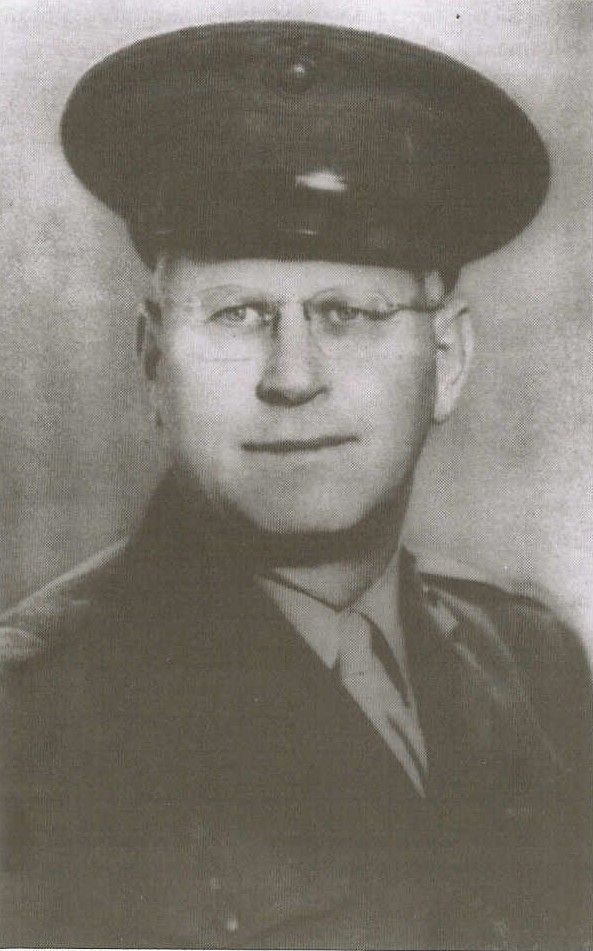
\includegraphics[width=0.13\textwidth]{pictures/Jonhston.jpg} 
	\end{figure}

    
    
%    \begin{itemize}
%    \item at 9 years old, he was  asked to  serve as an interpreter for a Navajo
%   delegation. 
%   \item WWI veteran.
%   \end{itemize}
\begin{itemize}
	\item 1942: he proposed to the Marine Corps that Navajos and
    other tribes could be recruited as code talkers.	

	   \item The major general Clayton
	    Barney Vogel accepted to try the idea.
\end{itemize}
    
\end{frame}
% ------------------------------------------------------------------------------------------------

\begin{frame}
    \frametitle{The demonstration}

    Johnston recruited four bilingual Navajos and % , on February 28,
    they went to Camp Elliott for a demonstration. 

    \begin{itemize}
    \item Two of the Navajos translated in Navajo typical military field orders
          and sent it by radio to their companions
    \item The companions translated the message in english.
    \end{itemize}
\end{frame}
% ------------------------------------------------------------------------------------------------


\begin{frame}
    Example, 

    \begin{quote}
    "Enemy expected to make tank and dive bomber attack at dawn." 
    \end{quote}

    becomes...
    \pause
    \begin{quote}
    "Enemy tank dive bomber expected to attack this morning." 
    \end{quote}
\pause
    Translation was done in 20 second instead of the 30 minutes needed by machines at that time.
\end{frame}
% ------------------------------------------------------------------------------------------------

    
\begin{frame}

    \begin{itemize}
    \item May 1942: 29 Navajos recruit task develop a Navajo code.
    \item Altogether, between 375 to 420 Navajos participated to the program. 
    \end{itemize}

    %![the letter](pictures/letter.jpg)
\end{frame}
\begin{frame}
    \frametitle{Efficiency of the Navajos code talkers}
 
	Battle of Iwo Jima:
	\begin{itemize}
	\item six Navajo Code Talkers were operating continuously. They sent more than 800 messages. All of the messages were transmitted without error.
    \end{itemize}
\begin{quote}
" Were it not for the Navajos, the Marines would never have taken Iwo Jima."
	\par
Major Howard Connor, signan officier of the Navajos at Iwo Jima
\end{quote}
	      
	      \pause
	\begin{itemize}
	\item
		They also served during the Korean War and at
the beginning of the Vietnam War.
\pause
\item According to the NY times, the Navajo code is the only spoken military code
never to have been deciphered.
	\end{itemize}

\end{frame}
% ------------------------------------------------------------------------------------------------

\begin{frame}
\section{Navajo and Navajo code}
    \begin{itemize}
	\item Why the Navajo language was a good choice
	\item How the code works
	\item Some flaws of the code
	\item Some evolutions of the code
    \end{itemize}
\end{frame}
% ------------------------------------------------------------------------------------------------

\begin{frame}
	\frametitle{Why the Navajo language was a good choice?}
    	\begin{itemize}
	\item<1-> The largest population of Native American so the possibility to recruit and
	  form enough code talkers

	\item<2-> It remained mostly "unwritten".
	\item<3-> Except the Navajos, only a handful of American experts were
		able to speak this language. 	
 	\item<4-> Navajo has a complex grammar, different from German and Japanese 
	\item<5-> faster than any machine at this time.
	\item<6-> Extremely difficult to distinguish for uninitiated Navajo Speakers
	\item<7-> Imposture aren't easy to make: it requires to speak Navajo with a good accent.
    \end{itemize}
\end{frame}
% ------------------------------------------------------------------------------------------------

\begin{frame}
    \frametitle{How it works}
    Because of a lack of military terms in the Navajo language, there was the need
    for a code which consisted in two different parts:
    \begin{itemize}
	\item Dictionary for common military words    
    \end{itemize}

\begin{center}
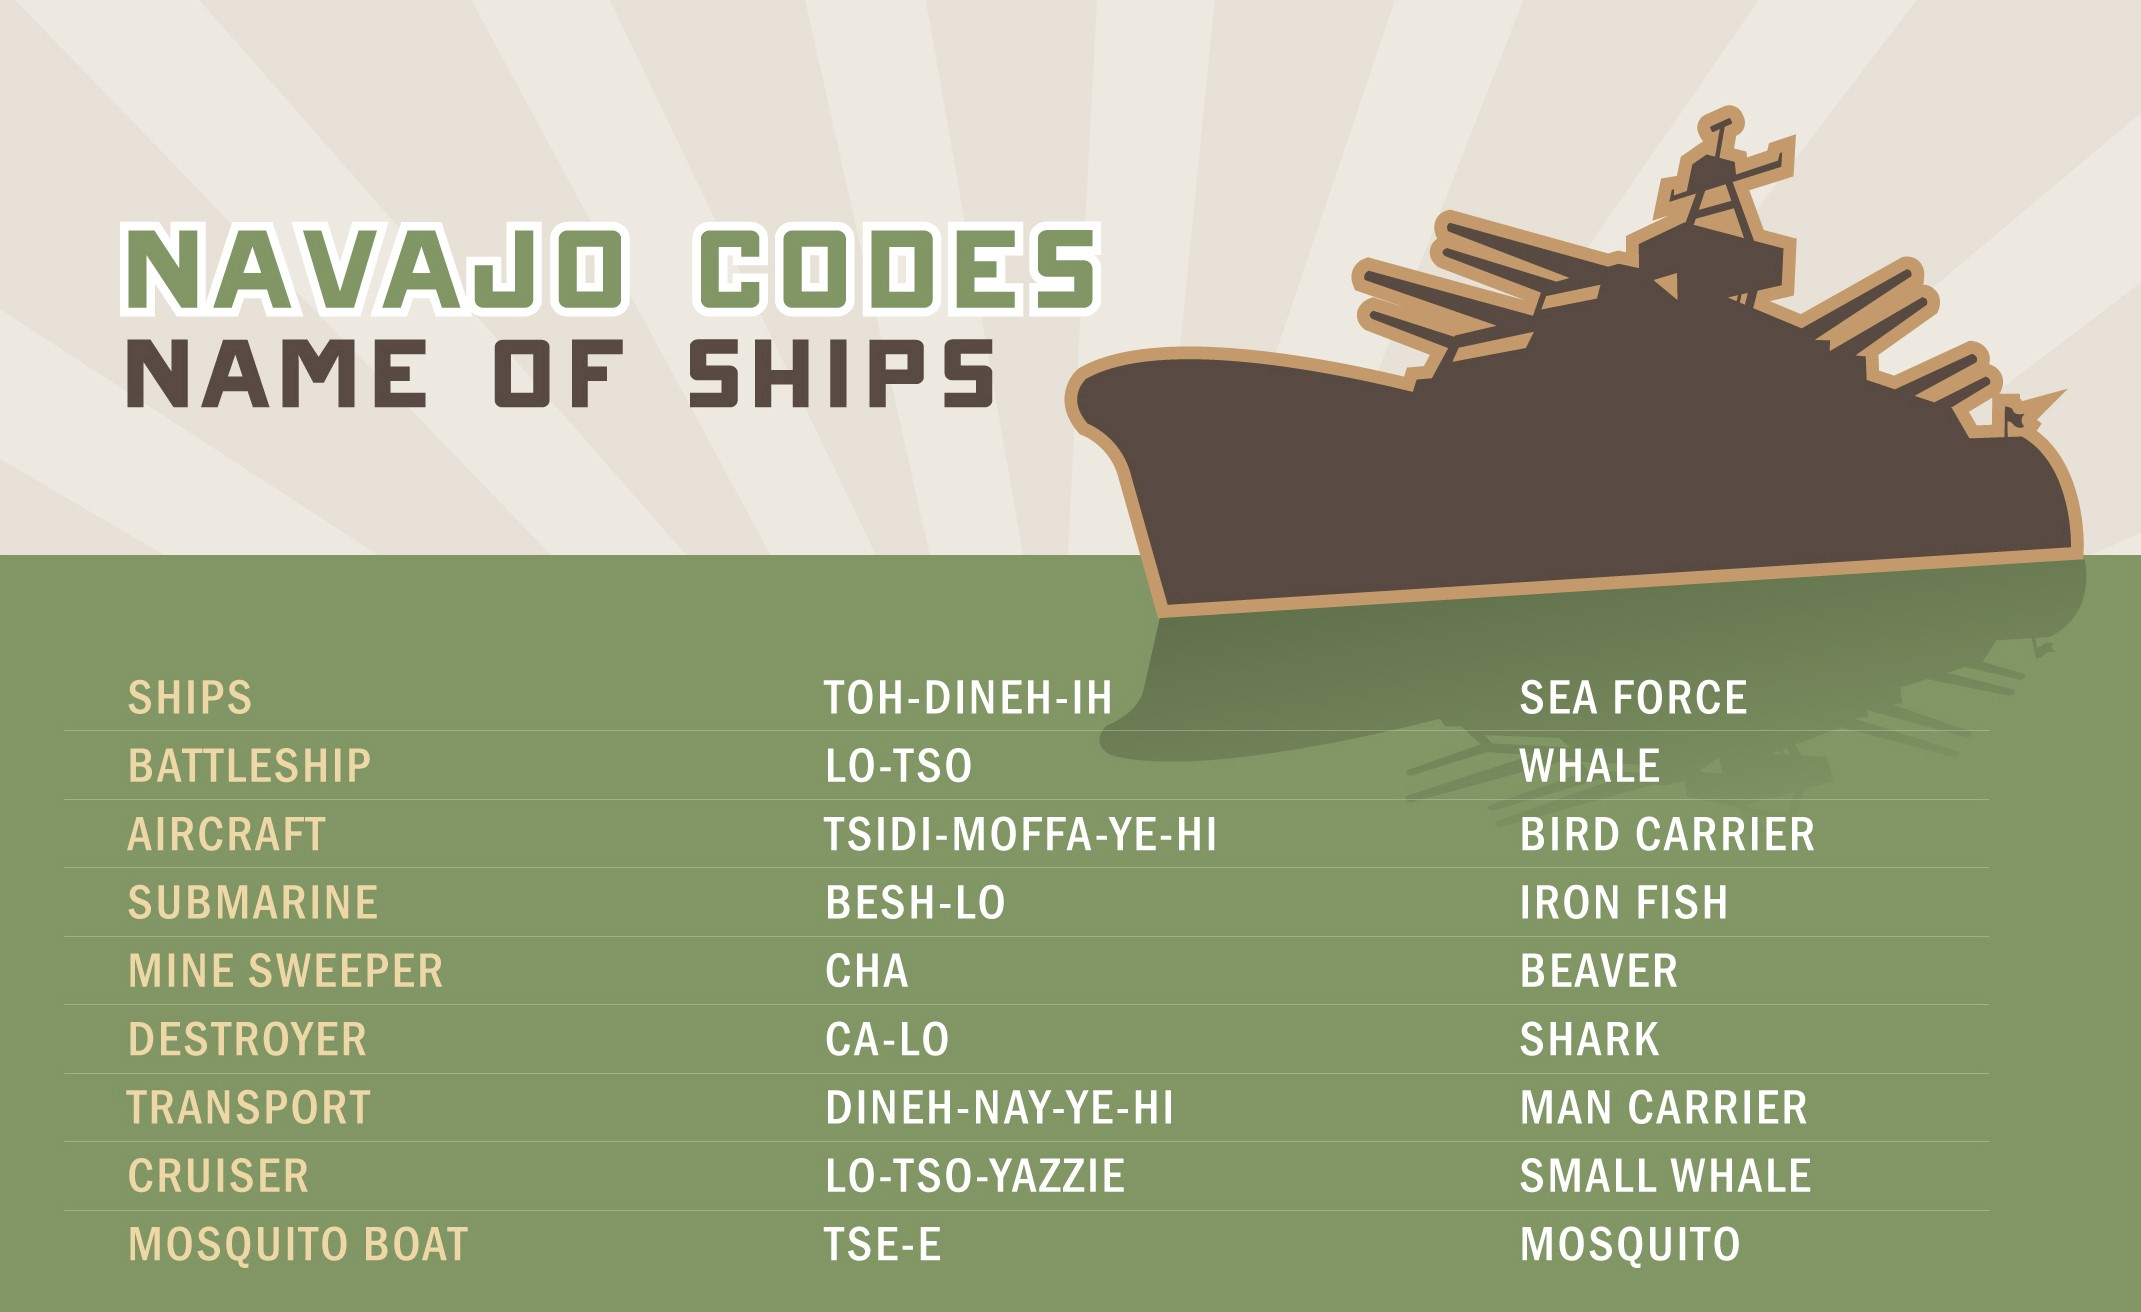
\includegraphics[width=0.7\textwidth]{pictures/ships.jpg} \newline
    \tiny{https://www.cia.gov/news-information/featured-story-archive/2008-featured-story-archive/navajo-code-talkers/}
\end{center}
\end{frame}
% ------------------------------------------------------------------------------------------------

\begin{frame}
    \frametitle{How it works}

    \begin{itemize}
    \item A phonetic alphabet table
    \end{itemize}

\begin{center}
    \begin{figure}[H]
\begin{tabular}{c|c|c}
\hline
A & WOL-LA-CHEE & Ant \\
\hline
B & NA-HASH-CHID & Badger \\
\hline
C & MOASI & Cat \\
\hline
D & CHINDI & Devil \\
\hline
E & AH-JAH & Ear \\
\hline
F & MA-E & Fox \\
\hline
\end{tabular}
	\caption{correspondance for some letters}
\end{figure}
	\tiny
	{https://www.cia.gov/news-information/featured-story-archive/2008-featured-story-archive/navajo-code-talkers/ }
\end{center}

%	      eagles, hawks, and all those domestic animals. Why don�t we use those names
%	      of different animals�from A to Z. So A, we took a red ant that we live with
%	      all the time. B we took a bear, Yogi the Bear, C a Cat, D a Dog, E an Elk, F,
%	      Fox, G, a goat and so on down the line.�Chester Nez, Navajo Code Talker,
%	      National Museum of the American Indian interview, 2004

\end{frame}
% ------------------------------------------------------------------------------------------------

\begin{frame}
    \frametitle{How it works}
	      \begin{itemize}
              \item Navajo Code Talkers memorized 17 pages of code during their training.
	      \item It was easier because of their culture of oral
		      transmission.
	      \end{itemize}
	      
	      A code talker answered one of his officers who had asked
	      why Navajos were able to memorize the complex code so quickly: 
	      
	      \begin{quote}
	      For us, everything is memory, it is part of our heritage. We have no written language.
	      Our songs, our prayers, our stories, they are all handed down from grandfather
	      to father to children and we listen, we hear, we learn to remember
	      everything. It is part of our training.\par
		  
	      (Power of a Navajo: Carl Gorman, the
	      Man and His Life, by Henry and Georgia Greenberg,1996) 
	      \end{quote}
\end{frame}
% ------------------------------------------------------------------------------------------------

\begin{frame}
    \frametitle{Some flaws of the code}
	About the code itself:
    \begin{itemize}
	\item<1-> Kerckhoffs's principles aren't observed.
	\item<2-> Non uniqueness of the translations on a message.
    \end{itemize}
	In practice:
    \begin{itemize}
	\item<3-> Navajos trained at different times and places so they
		develop different evolutions of the code.
	The solution to this flaw 
	was to frequently exchange Navajos from one division into another.
	\item<4-> There was not enough code talkers and some battalions
		remained without the capacity to decrypt and encrypt messages.
    \end{itemize}


	      
\end{frame}
% ------------------------------------------------------------------------------------------------

\begin{frame}
    \frametitle{Evolution of the code}
    \begin{itemize}
	\item The original dictionnary of 211 terms has been progressively 
	expanded to 411.
	\item  Multiple words to spell one letter.
    \end{itemize}

    \begin{center}
    \begin{figure}
    \begin{tabular}{c|c|c}
	\hline
	A & WOL-LA-CHEE & Ant \\
	\hline
	A & BE-LA-SANA & Apple \\
	\hline
	A & TSE-NILL & Axe\\
	\hline
    \end{tabular}
	\caption{multiple correspondances for one letter}
    \end{figure}
	\tiny
	{https://www.cia.gov/news-information/featured-story-archive/2008-featured-story-archive/navajo-code-talkers/ }
    \end{center}
\end{frame}
% ------------------------------------------------------------------------------------------------




\begin{frame}
\section{Conclusion:}
\end{frame}
% ------------------------------------------------------------------------------------------------
 
\begin{frame}
\frametitle{Declassification and recognition of code talkers after the war}
The program has been classified until 1968.

 
Recognition of code talkers:
\begin{itemize}
	\item 2000: the US Congree passed legislation to honor the Navajo Code Talkers
	  and give them special gold and silver congressional medals.
	\item 2008: the Code talkers recognition act was signed into law by president
	  George W. Bush, which recognizes every other native american code talker who served
	  in the United States military during WWI or WWII 
\end{itemize}

\pause
But there is still some lack of respect...
    \begin{itemize}
      \item 2017: during a White House event intended to honor the Navajo 
	 code talkers, Trump used the nickname "Pocahontas" to deride Elizabeth 
	 Warren, a political opponent.
    \end{itemize}
\end{frame}
% ------------------------------------------------------------------------------------------------

\begin{frame}
    \frametitle{Sources used}
    \begin{itemize}
    \item  https://www.archives.gov/education/lessons/code-talkers
    \item https://navajocodetalkers.org/
    \item https://www.cia.gov/news-information/featured-story-archive/2008-featured-story-archive/navajo-code-talkers/
    \item https://en.wikipedia.org/wiki/Code\_talker
    \item http://www.historynet.com/world-war-ii-navajo-code-talkers.htm 
    \item https://www.nytimes.com/2014/06/06/us/chester-nez-dies-at-93-his-native-tongue-helped-to-win-a-war-of-words.html?\_r=0)
    \end{itemize}
\end{frame}
% ------------------------------------------------------------------------------------------------

\end{document}
